\documentclass[a4paper,fleqn]{article}
\usepackage{iemss}
\usepackage{times}
\usepackage{graphicx}
\usepackage{natbib}
\bibpunct{[}{]}{;}{a}{,}{,~}
\usepackage{multirow}
\usepackage{float}
\usepackage{subfig}
\pagestyle{IEMSSheadings}
% Text to appear in the header of the pages
\IEMSShead{Stefanescu et al. / DEM uncertainty propagation}

\newcommand{\Pic}[2][0.85]{\begin{center}\includegraphics[width=0.8\textwidth,height=#1\textheight,keepaspectratio]{#2}
 \end{center} }


%\title{DEM uncertainty propagation and their impact on a geophysical flow model}

\title{DEM uncertainty and hazard analysis using a geophysical flow model}

%Authors Names and Affiliations:  Two spaces below the title, 10 pt
%Times Roman, Upper and Lower Case, underline author presenting
%paper and  provide his/her email address

\author{\underline{E.R. Stefanescu} \address[A1]{\it{Department of
Mechanical \& Aerospace Engineering, University at Buffalo, SUNY,
Buffalo,NY 14260 , (ers32@buffalo.edu, abani@buffalo.edu)}}, M.
Bursik\address[B1]{\it{Dept. of Geology, University at Buffalo, SUNY,
Buffalo,NY 14260 , (mib@buffalo.edu)}}, K. Dalbey \addressmark[A1],
M. Jones \address[C1] {\it {Center for Computational
Research,University at Buffalo, SUNY, Buffalo,NY 14260}}, A.K.
Patra\addressmark[A1] and E.B. Pitman\addressmark[A1] }

\begin{document}

\begin{abstract}
In this paper we introduce a careful procedure for analyzing the impact of 
error and uncertainty in model inputs in volcanic mass flow hazard analysis.
In particular we focus on uncertainty in elevation maps that are
crucial to flow simulations. Our early results establish the soundness
of the approach and the usefulness of the methodology for constructing
probabilistic hazard maps.
\end{abstract}
\begin{keyword}
  granular flow, computer model, TITAN2D, hazard map, probabilistic
\end{keyword}

\maketitle


\section{Introduction}

The aim of this study is to investigate the effect of Digital Elevation Model (DEM) uncertainty
on hazard analysis using a geophysical flow model.  In recent work
\citep{dalbeyjgr,dalbeythesis}, we have shown that input (e.g. volume)
and parameter (e.g. basal friction) uncertainty propagation through a
geophysical mass flow model can be used for analysis of hazards from
such flows. We follow up on that work here by exploring the impact of
uncertainty in DEM on the hazard analysis
application. The DEM, as the name implies, is a model of the elevation
surface. However, the DEM is often not treated as a model, but is
accepted as a ``true'' representation of the earth's surface
\citep{Suzanne_Wechsler}. The quality of a DEM is dependent upon a
number of factors, including the methods of data acquisition, the
nature of the input data, and the methods employed in generating the
DEMs \citep{Shearer_1990}.
Error is quantifiable, and is defined as the difference between
reality and our representation of the reality. Measurement of error
in DEM's is often impossible because the true value for every
geographic feature or phenomenon represented in a dataset is rarely
determinable \citep{Goodchild_1994, Hunter_1995}. Since the reality is
unknown, then the error can be characterized by methods commonly used
to treat epistemic uncertainty. In a geophysical flow model, the
uncertainty is the measure of the sensitivity of the analysis result
to variations of the parameters involved in it. Naive approaches to
treating DEM uncertainty can quickly lead to the use of thousands if
not millions of random variables, leading to a computationally
infeasible problem. We advocate instead a procedure introduced by
\citep{Goodchild_1994, Hunter_1995} that allows us to provide a
reasonable representation of DEM uncertainty using only one or two
random variables.

\subsection{Previous work}

A method use by \citep{Qihao_Weng} in quantification of the
uncertainty of DEMs was to create various DEMs using different
interpolation methods and to examine the RMSE from the source map,
sampling and measurement error, and interpolation process. It was
concluded that RMSE can be used as a general indicator of DEM
uncertainty.  \citet{Suzanne_Wechsler} developed four different
methods for representing the spatial dependence of error through
random fields to assess the effect on topographic parameters of the
DEM uncertainty. The study shows that uncertainty in the DEM is
manifested at higher elevations in local steeper slopes on the slope
and elevation maps.  Lower valley areas are more sensitive to error in
the data in the upslope contributing area map since error in lower
areas incorporates all the upslope area error.
One key feature of spatial data is the autocorrelation of observations
in space.  Generally, spatial autocorrelation refers to the
correlation between the same attribute at two locations. Observations
in close spatial proximity tend to be more similar than are
observations at greater separation. Errors in spatial data (such as
incorrect elevation values assigned to a point) are spatially
autocorrelated. The effect of correlated DEM error has been
investigated in a growing literature \citep{Fisher_1991,
Goodchild_1992}. It was determined that not only is error spatially
variable throughout a DEM, but within the elevation model the error
value of an individual grid cell is related to the error in
neighboring cells. Unfortunately, DEM providers do not furnish
information regarding the spatial dependence or spatial relationship
of errors.
Stochastic modeling uses stochastic conditional simulation to generate
multiple equally likely representations of an actual terrain
surface. \citet{Hunter_Goodchild_1997, Ehlschlaeger_1996} compute a
normal distribution of maps or realizations to reproduce the spatial
autocorrelation encountered in the original error surface, filtered
using a Gaussian convolution filter, with kernel sizes derived from
autocorrelation analysis of the original error surfaces. The technique
does not ensure that the ``real'' map is generated from the process;
however, it does provide a bound within which we can state the true
map lies.
Various researchers have applied the stochastic technique to evaluate
uncertainty in DEM data. \citet{Ehlschlaeger_1996} stochastically
simulated error in a DEM to evaluate the impact of DEM uncertainty on
a least-cost-path application. \citet{Hunter_Goodchild_1997}
investigated the effect of simulated changes in elevation at different
levels of spatial autocorrelation on slope and aspect
calculations. \citet{Felix_Hebeler} produced uncertainty surfaces to
show the impact of DEM uncertainty on an ice sheet
model. \citet{Amii_Darnell} developed a fuzzy framework to examine the
probable and possible uncertainties in classifying landslide hazard.



\subsection{TITAN2D model}

The TITAN2D code used in this effort conducts numerical simulations of
flows on digital representations of the natural terrain.  It is based
on a depth-averaged model for an incompressible granular material,
governed by Coulomb-type friction interactions \citep{Savage1989}.
The governing equations are obtained by applying conservation laws to
the incompressible continuum, providing appropriate constitutive
modeling assumptions, and then taking advantage of the shallowness of
the flows (flows are much longer and wider than they are deep) to
obtain simpler depth-averaged representations \citep{Patra2005}. The
motion of the material is considered to be gravitationally driven and
resisted by both internal and bed friction. The stress boundary
conditions are: no stress at the upper free-surface and a Coulomb-like
friction law imposed at the interface between the material and the
basal surface. Note that the primary factor driving the flow is the
component of gravity along the surface which depends on a local slope
computed from the elevation data.  Hence, the criticality of the DEM
to the flow computations. The resulting hyperbolic system of equations
is solved using a finite-volume scheme with a second-order Godunov
solver. Although many real geophysical flows --- such as debris flows
--- are fluidized, in this study we deal only with granular material
that has not been fluidized, such as dome-collapse block and ash flows
or rock avalanches initiated by slope instability.
The program runs in parallel, using the message passing interface
standard (MPI) to allow communication between multiple processors,
increasing computational power, decreasing computational time and
allowing use of large datasets. The algorithm uses local adaptive mesh
refinement for shock capturing, and dynamic load balancing for the
efficient use of computational resources. Topographic data are
included in the simulation by using a preprocessing routine in which
digital elevation data are imported. The DEM file containing $(X, Y,
Z)$ data (typically UTM easting, UTM northing and elevation in meters)
must be properly configured to operate with TITAN2D through the use of
a header. The DEM file containing $(X, Y,
Z)$ data (typically UTM easting, UTM northing and elevation in meters)
must be properly configured to operate with TITAN2D through the use of
a header.

\section{Stochastic simulation}

In modeling the propagation of uncertainty in a geophysical flow
model, the stochastic model proposed by \citet{Ehlschlaeger_1996} was
performed. The model is based on the observation that if an error
field can be defined by the available quantitative descriptors of
error, then its impact can be examined by simulating one or more
random error fields consistent with the available descriptors. Each
simulated field is a realization of the error model and the spatially
autocorrelated error can be viewed as a random field.
Two 30-m resolution DEMs derived from independent techniques were
used. An Shuttle Radar Topography Mission (SRTM) dataset was considered to be the ``true'' elevation,
while a second National Elevation Dataset (NED) dataset was used in creating the error model. To
find the error in a given DEM dataset the elevation given by the DEM
may be subtracted from the ``true'' elevation at a given
location. Random fields are then created based on the stochastic
properties of the difference dataset such that they are
representations of a potential realization of the errors in the map.
To choose the best descriptive parameters of a random field (the
minimum distance of spatial independence, the correlated distance
decay exponent and the filter parameter), a correlogram comparison of
the random field with the error model was performed. Sixty-four (64)
realizations were generated with a Gaussian distribution matching the
mean and standard deviation observed in the difference map represented
by \citep{Ehlschlaeger_1996}:
\begin{equation}
 R(\textbf{u})=m(\textbf{u})+m(m(T))+(m(s^2(T))\cdot \epsilon)\cdot Z(\textbf{u})
\label{eq:one}
\end{equation} 
where $R(\bf{u})$ is a realization of a generalized elevation dataset
$m(\bf{u})$,  $m(\bf{u})$ in this case is the SRTM dataset, $T$ is a group of sets
 of spatially uncorrelated sample
points, $\epsilon$ is a random variable with mean 0.0 and variance
1.0, and $Z(\bf{u})$ is the random field which captures the
autocorrelation between points.  The mean and the standard deviation
are determined from randomly drawn, spatially independent points
scattered across the surface.
The straightforward way to account for uncertain inputs and stochastic
forcing is a Monte Carlo approach --- run many simulations and
`average' the results in some fashion. If simulations are expensive to
run, this approach is not feasible. To circumvent this difficulty, the
statistics community has developed the idea of an emulator, or ``fast
surrogate'', computer model.  In essence, the emulator is a regression
surface based on a representative sample of simulations at selected
inputs, accompanied by statistical error bounds. Equipped with this
surface, output values at new (untested) input values need not be run.
Instead output results can be determined by evaluating the
emulator. There are indeed many methods -- kriging, metamodels,
support vector machines, etc., by which such surrogates may be
constructed and there exists a body of literature on the topic
\citep{simpson1,simpson2}.
One often-used emulator is the GAuSsian Process (GASP) emulator, which
assumes the regression has the form of a trend plus a Gaussian
\citep{kennedy2001bcc,ContiOHagan,ohagan2006bac,bayarriusc}.  To
construct a GASP emulator, the covariance structure of the Gaussian
must be assumed and parameters determined by Bayesian or partially
Bayesian methodology.  A fully Bayesian determination of the emulator
can be costly, especially if the input data is high-dimensional.  Here
we use the Bayes Linear method (BLM) \citep{blm1tutor} to construct an
emulator. Given prior beliefs $(B)$ of mean and variance, the BLM
updates these beliefs conditioned on the data $(D)$. \footnote{Note
that ``data'' here can refer to the output of expensive physics based
simulators.} Because only the first two moments of a distribution are
determined, the BLM is exact only for Gaussian distributions.  As an
emulator construction, the BLM update is simplier than a full GASP
construction, but the resulting emulator is comparable.  Given the
prior expectation $E[B]$ and variance $var(B)$, the BLM updates are
\begin{eqnarray} \label{blupdate}
E_D(B) &=& E[B] + cov(B,D) (var(D))^{-1} [D-E[D]] \\ \nonumber
var_D(B) &=& var(B) - cov(B,D) (var(D))^{-1} cov(D,B)
\end{eqnarray}
These update formulae can be derived by minimizing the mean square
error $(B - a^T D)^2$ between $B$ and some linear combination of the
data. Thus the BLM update can be viewed as the projection of the set
of prior beliefs onto the span of the data.


\section{Hazard Map Construction}

The next step of the analysis is to generate a functional
representation of the hazard at a location.  We describe the process
of computing a hazard map due to a geophysical flow with uncertain
model inputs introduced by \citet{dableyetalemulator,dalbeythesis}. A two-level construction of an
ensemble of emulators is used to include a separation of uncertain
inputs and geographic coordinates. The process starts by identifying
the model inputs whose uncertainties will drive the process. In our
case, the uncertain flow inputs we use are input volume, starting
location, basal and internal friction and finally the DEM.  For the
eight-dimensional parameter input space, a Latin Hypercube Sampling is
performed to determine parameter values at which simulations are to be
run. Simulation outputs at each of these parameter values are stored
at perhaps ($\mathcal {O} (10^6)$) grid points. This dataset is
downsampled to tens of thousands of grid locations.  The variable of
interest for our application is the single field of maximum flow depth
over time, at each of the downsampled gridpoints.  Tesselations of the
geographic coordinate space and the parameter input space are
constructed (we use Delaunay triangulation).  At a designated
location, ${\bf x}^*$, of the input plus coordinate space at which the
hazard is to be computed, the covering simplex $S_{\bf x}^* $ of the
parameter space is identified, and all nodes of that simplex are
enumerated, as are all nodes within a neighborhood (two hops in the
tesselation) of the covering nodes.  For each such 2-hop node, we
tesselate in the geometric coordinates and evaluate all emulators
constructed over these nodes (standard BLM emulators).  We average
these coordinate space emulators to (the coordinate components of)
${\bf x}^*$ by barycentric weighting; notice there will be emulators
for each parameter input sample point. Now in the input parameter
space, construct a tessellation of the 2-hop nodes and average the
emulators to ${\bf x}^*$ by barycentric weighting of the fine scale
emulator.  The emulator is now readily and quickly evaluated (at the
cost of a few FLOPS) for each evaluation. The hazard map construction
can now proceed by treating the emulator as a surrogate for the
simulator in the classical Monte Carlo procedure. For any point in the
domain now we can exercise the emulator to get potential flows and
hence exceedance probabilities.

\section{Application}
\subsection{Study site}

The study area is Mammoth Mountain --- a large, geologically young,
composite dome volcano located on the southwestern rim of Long Valley
Caldera, California \citep{Bailey1989}.  There are many active hazards
issues for Mammoth Mountain, including snow avalanches, rock
avalanches and debris flows. In addition, it is intersected by the
Mono-Inyo Craters volcanic chain, which is the most active volcanic
region in the southwestern U.S.  If Mono-Inyo type activity occurs on
Mammoth Mountain, then domes may form.  These new domes would be
growing atop a steep edifice, and therefore could become
gravitationally unstable.  Given that block and ash flows occurred at
Mammoth Mountain during its older dome growth stage, there is reason
to believe that renewed dome formation would result in block and ash
flow activity. If this is so, then parts of Mammoth Lakes, CA, are at
risk from block and ash flows.  Our previous work on Mammoth Mountain
(Stefanescu et al., submitted) was the the testing of the hypothesis
that different DEMs result in different model outputs. One of the most
important conclusions was that for moderate and smaller scale flows it
is important to capture the terrain's features in order to get an
accurate footprint of the flow.

\subsection{DEMs and Uncertainty in DEMs}

A rectangular area of approximative 42 kilometers$^2$ was defined
within the SRTM and NED DEMs (Fig.~\ref{fig1} a). The correlogram for the data 
was calculated to determine the range of spatial dependence of the elevation points using
Grass GIS functions. We found that the spatial dependence persisted to a distance of 2000 meters.
To determine the PDF for the stochastic simulation, 91 sets of spot locations were selected from the 
area covered, each set containing 91 points, all separated by more than 2000 meters. For each set,
PDF statistics (mean and standard deviation) were derived (Fig.~\ref{fig1} b). An important step in
the analysis is to determine the random field parameters, which
required the development of many combinations of spatial dependence
parameters. After testing more than 600 random field parameter, the
combination which resulted in the smallest difference between the
error model correlogram and the random field is: the minimum distance
of spatial independence, $D =2100$; the distance decay, $E = 0.7$, and
the filter parameter, $F =350$. A total of 64 equally probable
potential elevation surfaces of the area having a 30-m resolution were
generated.

%Put picture of DEM and error model here -- list parameters chosen for errror model -- D, F, exponent ...

\subsection {Parameters, Uncertainty, and Probabilistic Hazard Maps}

The central concept guiding the creation of hazard maps for volcanic
eruptions, as well as earthquakes, floods, etc., is that volcanoes
tend to behave in the future in a manner that is similar to how they
have behaved in the past. Thus, the geological record can be used by
volcanologists to estimate quantities that parameterize past flows,
and even probability distributions for these parameters
\citep{dalbeyjgr,dalbeythesis}.  These parameter values can then be
used to guide modeling of potential future events.  If the input
values for a future event of interest were known exactly, then a
hazard map could be generated from a single simulation evaluated at
those input values. Since we lack knowledge of the future, it is
necessary to examine flow behavior over a range of inputs. Thus we
must choose which inputs to consider uncertain and their appropriate
ranges.
The motivation for creating realizations of the DEM was to be able to
use them along with other uncertain parameters as uncertain inputs for
a hazard map.  One of our assumptions is that the DEM contributes a
significant proportion of the variance in simulated flow, hence hazard
map output.  For sampling the input space, a Latin Hypercube Sampling
(LHS) was implemented.  The uncertain inputs of the hazard map in this
case were:
\begin{enumerate}
\item The DEM, which is
defined by two random variable with mean 0.0 and variance 1.0
\item The starting position of the initial unstable material, which is
uniformly distributed in a circle of radius 400 m, centered at
(322058,4167488)
\item The volume, which is uniformly distributed between a minimum
event of $10^5 m^3$ and a maximum event of $10^9 m^3$. 
\item  Internal friction angle, with values
in the range $[20 - 25]$ degrees
\item Basal friction angle, which was considered to have a uniform
distribution between $[15 - 20]$ degrees where the elevelation is
greater than 2750m, and below this $ [20 - 25]$.  This is the
elevation of the tree line; we are assuming that trees and greater
degree of soil development provide greater flow dissipation.
\end{enumerate}
The parameter values listed above were used to guide the LHS sampling
of the input space of potential block and ash flows in the future.
Outputs from TITAN2D model runs at the sampled input values were then
combined and analyzed to produce a probabalistic hazard map given
uncertainty in flow volume, topography, and dissipation.



\section{Discussion and Conclusions}

In our previous work \citep{stefanescu1}, we investigated the effects
of DEMs on the output of TITAN2D by comparing the output using
different DEMs to that obtained with a ``true'' representation of the
terrain, which is considered to be that obtained by using TOPSAR-5m
data.  We found that DEMs with different resolutions and sources
generated different outputs which led to different flow maps
(Fig.~\ref{fig2} (a), (b)).  A next step in studying the effect of DEM
on the flow depth output is to create multiple realizations of a
particular DEM and develop a hazard map which has as uncertain input
parameters the terrain realizations, volume, location and basal
friction.
Thirty-two (32) potential DEM realizations were created by adding to
the SRTM 30m DEM the difference between the two DEMs multiplied by a
random variable, $\epsilon$, with a mean of 0.0 and a variance of 1.0.
The realizations do not take into account the spatial autocorrelative
effect between points, but they do assume that the two DEMs are
consistent; there is a measurement error in both DEMs where it was
difficult to collect the raw data points, or where the slope angle was
steep. The distributions of uncertainty for all the input parameters
were propagated through the simulator to produce a map of the
probability that a hazard criterion -- in our case a flow depth of 0.2
m -- can be met (Fig.~\ref{fig3}).
We have introduced here a systematic procedure to use uncertainty in
model inputs (notably the DEM) and parameters to drive the analysis of
hazards from geophysical granular flows such as ignimbrites, block and
ash flows or avalanches.  As we had previously found in studying the
effects of input parameter uncertainty in only the physical flow
parameters (such as volume and friction angle) \citep{Keith}, error in
flow property output uncertainty is concentrated at the flow margins.
This is somewhat surprising in that DEM uncertainty is concentrated by
local errors in terrain surfaces.  The result may therefore indicate
that flow thickness plays a greater role in concentrating uncertainty,
which is preferentially concentrated at flow margins where the
material has thinned considerably.


\centerline{\it ACKNOWLEDGEMENTS}
This work was supported by NASA grant NNX08AF75G to study DEM
uncertainty on flow model output.  Referees are thanked for useful
comments and their time.



%\begin{figure}[H]
%    \begin{minipage}[b]{0.6\textwidth}
%        \begin{tabular}{c}
%        \Pic[0.3]{SRTM30_dem.jpg}\\
%        (a)
%        \end{tabular}
%    \end{minipage}
%%\hfill
%    \begin{minipage}{0.6\textwidth}
%        \begin{tabular}{c}
%        \Pic[0.3]{NED30_dem.jpg}\\
%        (b)
%        \end{tabular}
%    \end{minipage} 
%\caption{Low flow}
%\label{fig1}  
%\end{figure}

%

\begin{figure}[H]
    \begin{minipage}[b]{0.6\textwidth}
        \begin{tabular}{c}
       % \Pic[0.3]{SRTM30_dem.jpg}\\
	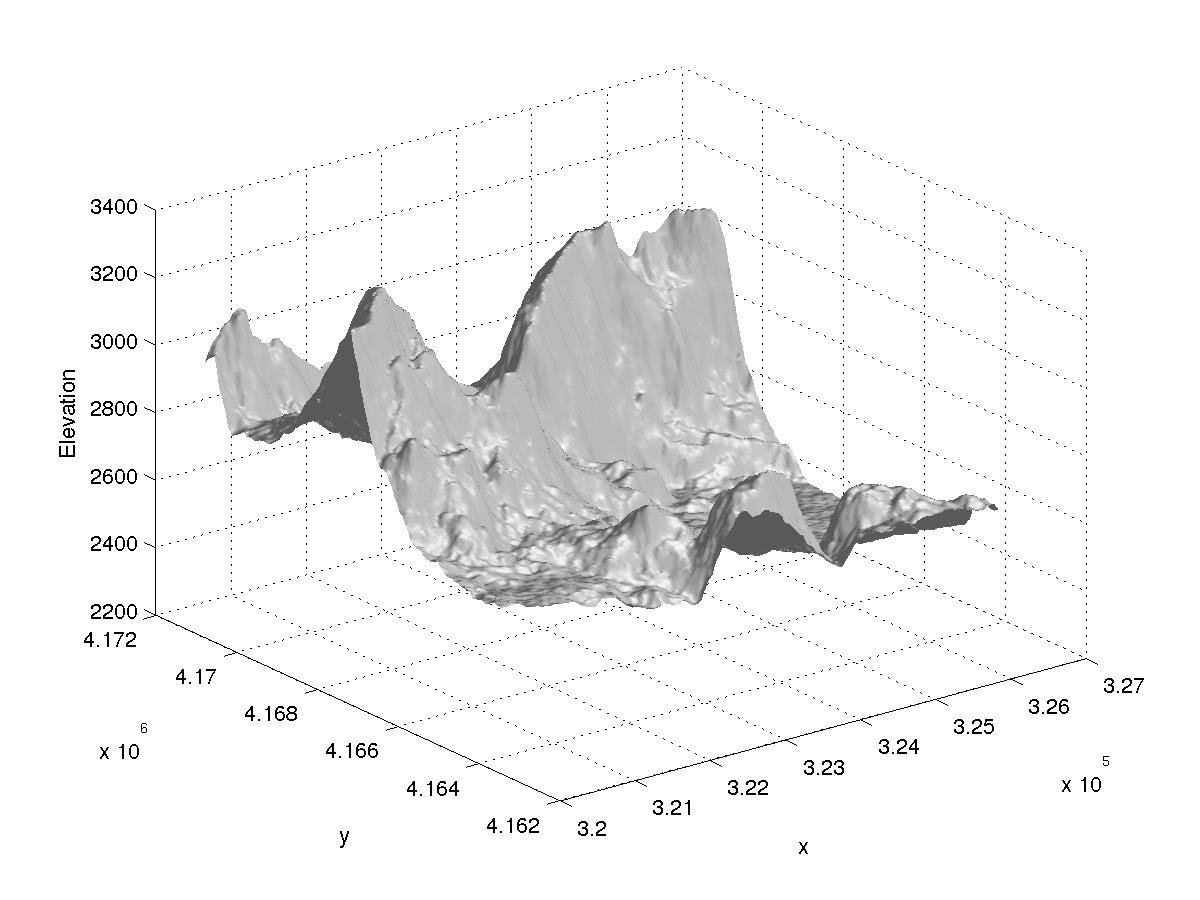
\includegraphics[width=7cm,height=8cm,keepaspectratio]{SRTM30_dem.jpg}\\
        (a)
        \end{tabular}
    \end{minipage}
%\hfill
    \begin{minipage}{0.6\textwidth}
        \begin{tabular}{c}
       % \Pic[0.3]{NED30_dem.jpg}\\
	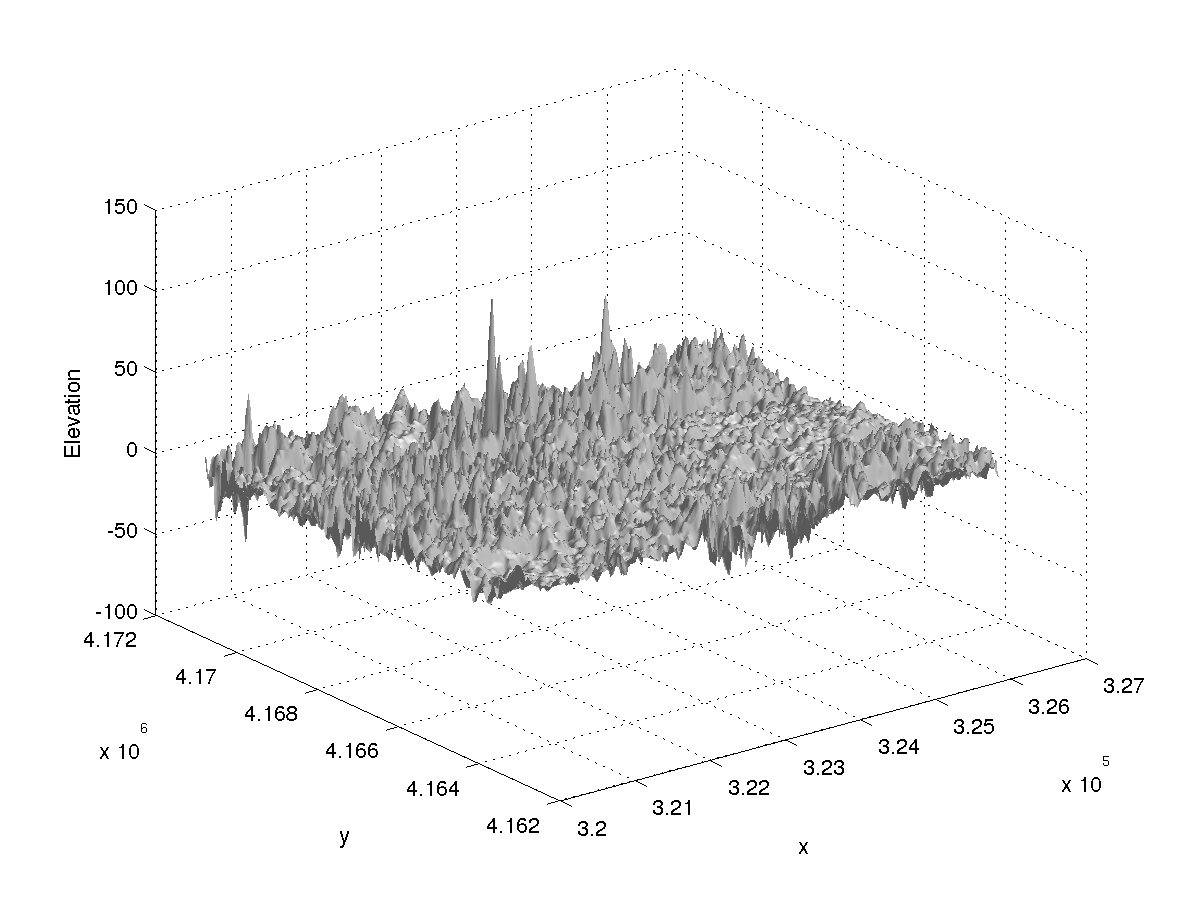
\includegraphics[width=7cm,height=8cm,keepaspectratio]{difference.jpg}\\
        (b)
        \end{tabular}
    \end{minipage} 
\caption{(a) The SRTM 30m DEM terrain surface (Easting, Northing and elevation coordinates). (b) Magnitude of the error model as measured by the 
difference between the two DEMs. }
\label{fig1}  
\end{figure}

\begin{figure}[H]
    \begin{minipage}[b]{0.6\textwidth}
        \begin{tabular}{c}
       % \Pic[0.3]{SRTM30_dem.jpg}\\
	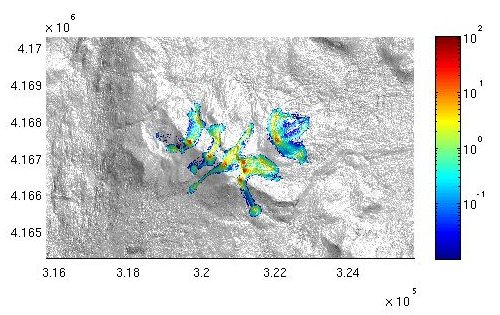
\includegraphics[width=7cm,height=8cm,keepaspectratio]{Mammoth_low.jpg}\\
        (a)
        \end{tabular}
    \end{minipage}
%\hfill
    \begin{minipage}{0.6\textwidth}
        \begin{tabular}{c}
       % \Pic[0.3]{NED30_dem.jpg}\\
	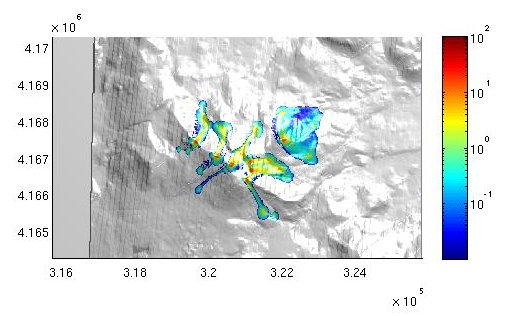
\includegraphics[width=7cm,height=8cm,keepaspectratio]{ned30_low.jpg}\\
        (b)
        \end{tabular}
    \end{minipage} 
\caption{a) and b) Examples of differences in flow depth calculations for realizations of the same low-volume flow using different DEMs. 
a) TOPSAR 5m DEM, b) NED 30m DEM}
\label{fig2}  

\end{figure}
\begin{figure}[H]
    \begin{minipage}[b]{0.6\textwidth}
        \begin{tabular}{c}
        %\Pic[0.3]{fig1.jpg}\\
	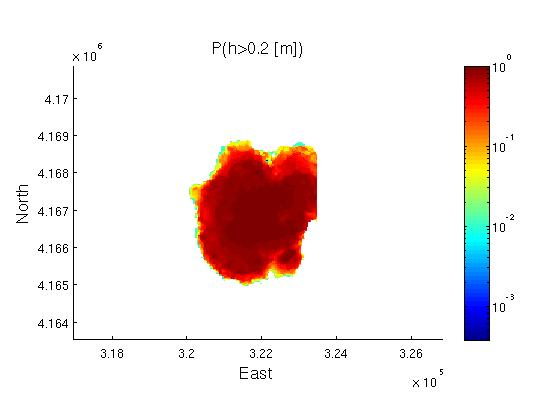
\includegraphics[width=7cm,height=8cm,keepaspectratio]{fig1.jpg}\\
        (a)
        \end{tabular}
    \end{minipage}
%\hfill
    \begin{minipage}{0.6\textwidth}
        \begin{tabular}{c}
       % \Pic[0.3]{fig2.jpg}\\
	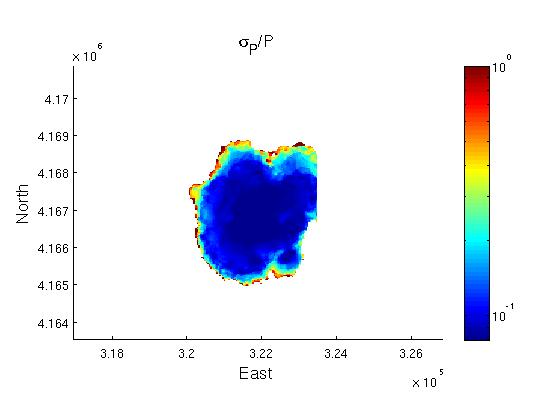
\includegraphics[width=7cm,height=8cm,keepaspectratio]{fig2.jpg}\\
        (b)
        \end{tabular}
    \end{minipage} 
\caption{a) Probability that a flow will exceed 0.2 m in depth as a function of position on Mammoth Mountain, CA, given the uncertainties in DEM and input parameters.
b) Standard deviation in the estimate that the flow will exceed 0.2 m in depth. Estimation error is concentrated at flow margins.}
\label{fig3}  
\end{figure}


%%%%%%%%%%%%%%%%%%%%%%%%%%%%%%%%%%%%%%%%%%%%%%%%%%%%%%%%%%%%%%%%%
\bibliographystyle{iemss}
\bibliography{iemss}
%%%%%%%%%%%%%%%%%%%%%%%%%%%%%%%%%%%%%%%%%%%%%%%%%%%%%%%%%%%%%%%%%

%  \bibitem{simpson1} T.W. Simpson, J.D. Poplinski, P. N. Koch and J.K. Allen,
%  Metamodels for Computer-based Engineering Design: Survey and recommendations,
%  Engineering with Computers,Volume 17, Number 2 2001

%\bibitem{simpson2}SM Clarke, JH Griebsch, TW Simpson
% Analysis of Support Vector Regression for Approximation of Complex Engineering Analyses
%J. Mech. Des.  -- November 2005 --  Volume 127,  Issue 6, 1077 (11 pages) 
%doi:10.1115/1.1897403

%\bibitem{dalbey2009psm}
%Keith~R. Dalbey.
%\newblock {\em {Predictive Simulation and Model Based Hazard Maps of
%  Geophysical Mass Flows}}.
%\newblock PhD thesis, Department of Mechanical and Aerospace Engineering,
%  University at Buffalo, April 2009.

%\bibitem{dalbeyjgr} K. Dalbey, A. K. Patra, E. B. Pitman, M. I. Bursik, and M. F. Sheridan, Input uncertainty propagation methods and hazard 
%mapping of geophysical mass flows 
%J. Geophys. Res., 113, B05203, doi:10.1029/2006JB004471.
%\bibitem{Hubbard2007clh}
%B.E. Hubbard, M.F. Sheridan, G.~Carrasco-N{\'u}{\~n}ez,
%  R.~D{\'\i}az-Castell{\'o}n, and S.R. Rodr{\'\i}guez.
%\newblock {Comparative lahar hazard mapping at Volcan Citlalt{\'e}petl, Mexico
%  using SRTM, ASTER and DTED-1 digital topographic data}.
%\newblock {\em Journal of Volcanology and Geothermal Research},
%  160(1-2):99--124, 2007.
%\bibitem{dableyetalemulator} K. Dalbey, M. Jones, E. B. Pitman, E. Calder, M. Bursik A. Patra
%Hazard Risk Analysis Using Computer Models of Physical Phenomena and Surrogate Statistical Models
%submitted to Comp. Meth. App. Mech. and Eng.
%
%\bibitem{bayarriusc}
%M.J. Bayarri, James~O. Berger, Eliza~S. Calder, Keith Dalbey, Simon Lunagomez,
%  Abani~K. Patra, E.~Bruce Pitman, Elaine~T. Spiller, and Robert~L. Wolpert.
%\newblock Using statistical and computer models to quantify volcanic hazards.
%\newblock to appear Technometrics, 2010.
%\bibitem{ContiOHagan}
%Stefano Conti and Anthony O'Hagan.
%\newblock Bayesian emulation of complex multi-output and dynamic computer
%  models.
%\newblock Research Report No. 569/07, Department of Probability and Statistics,
%  University of Sheffield. Submitted to Journal of Statistical Planning and
%  Inference. website:
%  \url{http://www.tonyohagan.co.uk/academic/ps/multioutput.ps}.
  







\end{document}
